\documentclass[11pt,a4paper]{article}

\usepackage{graphicx}
\usepackage{easrp2026}

\easrpauthor{Oleh Kovalyshyn, Yevhenii Zasko, Volodymyr Sydorskyi}
\easrpaffiliation{Kyiv School of Economics, Kyiv, Ukraine}

\easrptitle{Fine-tuning paths for 60-minute glucose forecasts:\\
a JEPA feature on a GluMind-style backbone}

\begin{document}

\maketitle

\begin{abstract}
A 60-minute continuous glucose monitor (CGM) forecast can be served from a
population model on day zero. Adapting that model to one person is usually
reported as two endpoints: zero-shot, and fine-tune on all available history.
The path between those points is the practical question. Short fine-tunes can
raise error, so a system needs a gate: keep the frozen weights until enough
days exist.

We specify SugarOne, a GluMind-style forecaster retargeted to commodity CGM
and insulin-record covariates, and SugarJEPA-288, which adds a CGM-JEPA
embedding as a fourth input stream. On a personal test split of seven T1DM
users, frozen SugarJEPA-288 has lower MAE than SugarOne fine-tuned for 30 days
for every user. SugarJEPA-288's own fine-tune path stays at or below its
zero-shot mean from 3 days onward and still improves at full history, with
the JEPA encoder held frozen. SugarOne and NBEATSx need a longer wait;
TFT helps by 30 days on average but is harmful at 3--14 days.

The study is small (\(n=7\) T1DM). Smoothness is an empirical check, not a
guarantee.
\end{abstract}

\section{Introduction}
\label{sec:intro}

A CGM reports an excursion after it has begun~\citep{rodbard2016cgm}.
A 60-minute forecast---12 steps at 5-minute sampling---is the task of this
paper. A population model can be served immediately. Personal history arrives
slowly. After \(N\) days of one person's data, is the fine-tuned checkpoint
safe to serve?

Glucose forecasting papers usually report a frozen global model, or one
adapted model trained on all available personal data, or both
\citep{sergazinov2022gluformer,zhu2023personalized}. They rarely show the
budgets in between. If 3--30 days of fine-tuning raise MAE, ``always adapt''
is the wrong rule. The system needs a gate: keep the frozen weights until
the path is no longer harmful.

This paper treats personalization as a \emph{curve}. We introduce
\textbf{SugarOne}: the GluMind parallel dual-attention design
\citep{farahmand2025glumind} retargeted to covariates a commodity CGM plus
an insulin record actually has (Section~\ref{sec:sugarone}). SugarOne has no
prior paper; it is specified here because it is the backbone we fine-tune.
\textbf{SugarJEPA-288} adds a CGM-JEPA embedding~\citep{muhammad2026cgmjepa}
as a fourth stream. We compare day-budget curves on the same seven T1DM
people against SugarOne and NeuralForecast continue-fit
\citep{neuralforecast2022,olivares2023nbeatsx,lim2021tft}.

Contributions:
\begin{itemize}
    \item SugarOne: GluMind blocks on commodity covariates, our
    hyperparameters, and a joined Loop + AI-READI corpus.
    \item Personalization scored as a path (zero-shot, then 3, 7, 14, 30, 60,
    and full history) with a named smoothness check.
    \item On this cohort, a JEPA feature raises the day-zero floor and keeps
    short fine-tunes non-harmful. Frozen SugarJEPA-288 beats 30-day SugarOne
    for all seven users.
\end{itemize}

\section{Related work}
\label{sec:related}

\paragraph{Glucose transformers.}
GluMind uses parallel cross-attention and multi-scale self-attention on
glucose, heart rate, and steps~\citep{farahmand2025glumind}. Gluformer and
related attention models forecast from CGM with optional
personalization~\citep{sergazinov2022gluformer}. We keep GluMind's block
design and change covariates, mixing, size, and training data
(Section~\ref{sec:sugarone}). We do not run a GluMind-versus-SugarOne
leaderboard.

\paragraph{Self-supervised CGM.}
CGM-JEPA learns glucose representations with a joint-embedding predictive
objective~\citep{muhammad2026cgmjepa}. We use that idea as an extra
\emph{supervised-forecast} stream, pretrained on our train split. This is not
a new foundation model.

\paragraph{Personalization and baselines.}
Fine-tuning and meta-learning for T1DM typically yield one adapted
model~\citep{zhu2023personalized}. GlucoBench standardizes public CGM
forecasting~\citep{sergazinov2024glucobench} but not day-budget adaptation
curves. We use NBEATSx and TFT, via NeuralForecast, as continue-fit
baselines~\citep{olivares2023nbeatsx,lim2021tft,neuralforecast2022}.

\section{Method}
\label{sec:method}

\subsection{Task}
\label{sec:task}

Each model maps a lookback window to the next \(H=12\) glucose values
(60 minutes). The lead metric is MAE in mg/dL. Tables also report RMSE and
MARD. The horizon is the same for every model.

\subsection{Data and two tests}
\label{sec:data}

Raw CGM and pump exports are resampled to a 5-minute grid and gap-filled
with \texttt{glucose\_data\_processing}~\citep{glucosedataprocessing}. We
vertically join AI-READI-style wearable CGM~\citep{aireadi2024} and Loop T1DM
pump records into one loop-style table (\texttt{loop\_ai\_ready\_joined2.csv};
12.1 million rows; about half T1DM / half non-T1DM by row mass). Study groups
are Healthy, Pre-T2DM, Oral-T2DM, Insulin-T2DM, and T1DM. AI-READI rows have
empty insulin and carbohydrate fields (zero-filled). Sequence IDs are prefixed
so the two sources cannot collide.

We use two evaluations. Mixing them is a wrong sentence.

\textbf{Global test.} The dataset \texttt{test} split of the joined table.
Question: is this a competent population model?

\textbf{Personal test.} Seven T1DM users with long history: one personal
pump export (Livia, \(\sim\)345 train days) and six Loop quality holdouts
(Users 154, 556, 730, 1017, 1029, 1082). Each person's CSV is split
chronologically: last 25\% test, 15\% of the remainder validation, the rest
train. A day budget shortens \emph{train} only. Validation and test never
change. User 1082 has \(\sim\)37 train days and no 60-day cell; 60-day means
use \(n=6\).

Eight short-wear AI-READI users (\(\sim\)6--9 train days, no insulin/carb
channels) are not in the main curve. SugarJEPA-288 needs a one-day lookback;
those series are a limitation, not a second cohort.

\subsection{SugarOne}
\label{sec:sugarone}

SugarOne uses GluMind's parallel dual-attention blocks
\citep{farahmand2025glumind}. A linear layer maps each scalar channel to
\(d_{\mathrm{model}}\) and adds sinusoidal positional encoding. Each block
has (i)~cross-attention in which glucose embeddings are queries and each
auxiliary supplies its own keys and values, and (ii)~multi-scale
self-attention on glucose at downsampling factors 1, 2, and 4. A two-layer
MLP decodes 12 steps.

GluMind was built for wearable extras. SugarOne is the same design aimed at
a commodity CGM plus an insulin record. Table~\ref{tab:glumind-vs-sugarone}
is the difference. Fusion is learnable softmax mixing over the three
auxiliary streams,
\[
\mathbf{C}=\sum_{i=1}^{3}w_i\mathbf{C}_i,\qquad
w_i=\frac{\exp(\alpha_i)}{\sum_{j}\exp(\alpha_j)},
\]
with \(\boldsymbol{\alpha}\) initialized at zero (equal mix). We do not evaluate a
GluMind checkpoint on the personalization curves. SugarOne is the control in
the same family as SugarJEPA.

\begin{table}[t]
\centering
\small
\begin{tabular}{lcc}
\toprule
 & GluMind & SugarOne \\
\midrule
Auxiliaries & Heart rate, steps & Basal, bolus, carbohydrates \\
Fusion & Fixed average & Learnable softmax \\
Lookback / size & 80 steps, 4 heads, 3 blocks & 128 steps, 8 heads, 5 blocks \\
Width & \(d=32\) & \(d=32\) \\
Training table & Wearable AI-READI-style & Joined Loop + AI-READI \\
\bottomrule
\end{tabular}
\caption{SugarOne is unpublished. It keeps GluMind's blocks and changes
covariates, mixing, size, and data.}
\label{tab:glumind-vs-sugarone}
\end{table}

\subsection{SugarJEPA}
\label{sec:sugarjepa}

We pretrain a CGM-JEPA-style encoder~\citep{muhammad2026cgmjepa} on the
joined \texttt{train} split, glucose only. A random 5\% of that split is held
out for encoder validation and is never used for encoder training. The loss
is SmoothL1 latent prediction plus an EMA teacher and a VICReg-style variance
penalty~\citep{bardes2022vicreg}:
\[
L=\mathrm{SmoothL1}(\hat{z},z)
+\lambda\frac{1}{E}\sum_{j=1}^{E}
\mathrm{ReLU}\bigl(\sigma_{\mathrm{target}}-\sigma_{c,j}\bigr),
\]
where \(E\) is the embedding size and \(\sigma_{c,j}\) is the standard
deviation of context-block representations on dimension \(j\).

The encoder is attached as a fourth SugarOne branch, on the same footing as
basal, bolus, and carbohydrates (Figure~\ref{fig:arch}). Embeddings are
layer-normalized and projected from 96 to 32 dimensions before
cross-attention. If the encoder wants \(m\) steps and SugarOne wants
\(n=128\), with \(m>n\), each training window has length \(m\): the encoder
sees all \(m\) points; SugarOne sees the last \(n\).

During \emph{global} SugarJEPA training the encoder is not frozen. It is
updated at \(4\times10^{-5}\); the rest of the model at \(4\times10^{-4}\).
The hero encoder is \textbf{jepa-288} (96 dimensions, 288 steps, one day of
CGM). Other windows (128, 864, 2016) are in Appendix~\ref{app:windows}.
Longer windows change which series can be scored; they are not the claim of
this paper.

\begin{figure}[t]
\centering
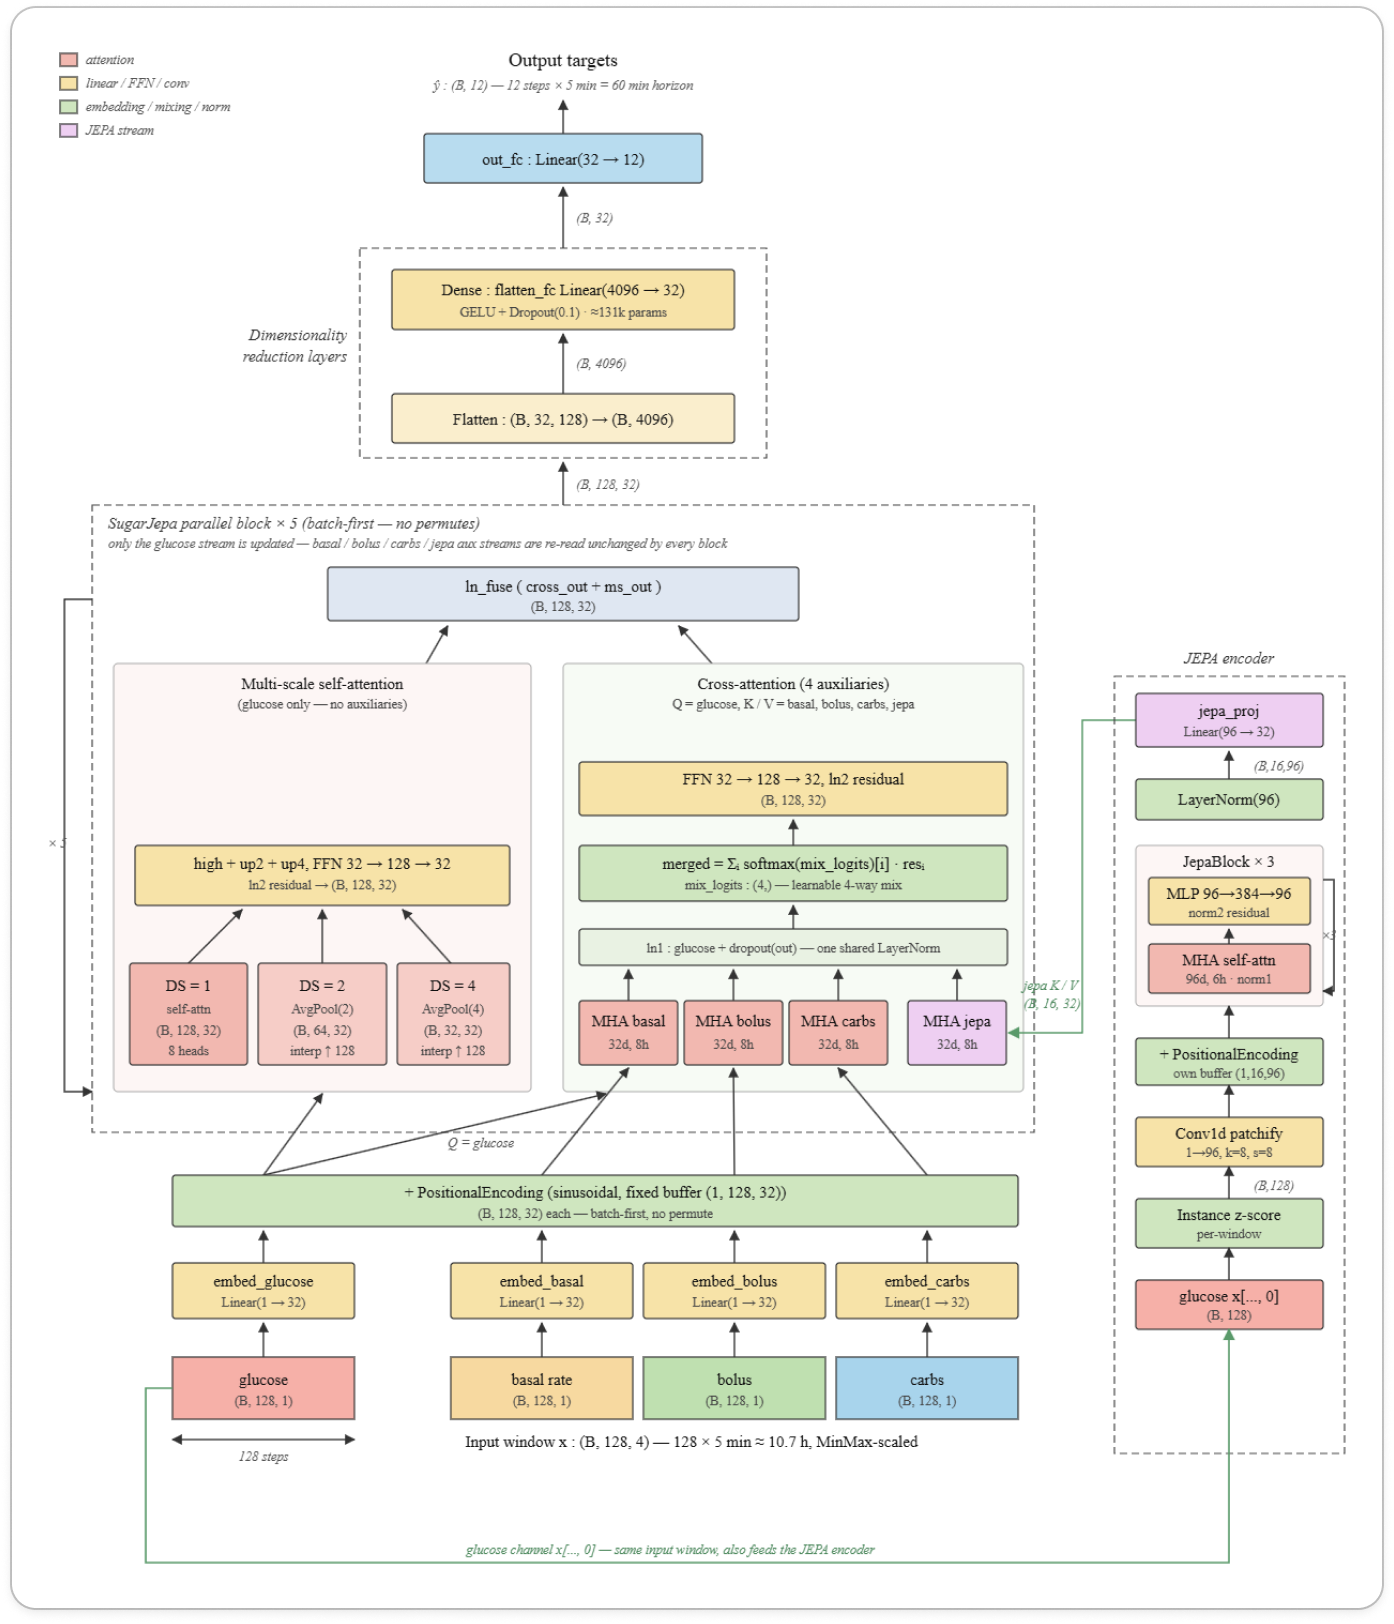
\includegraphics[width=0.82\textwidth]{sugar_jepa.png}
\caption{SugarJEPA: SugarOne branches (glucose, basal, bolus, carbohydrates)
plus a JEPA auxiliary. Personal fine-tunes freeze the encoder and update the
SugarOne weights.}
\label{fig:arch}
\end{figure}

\subsection{Fine-tune protocol and smoothness}
\label{sec:protocol}

Each day budget is an independent run from the global checkpoint, not a
curriculum. Scalers stay the global \texttt{scalers.json}; they are not
refit on personal train. SugarJEPA personalization freezes the JEPA encoder
and updates only the SugarOne weights. We use plain fine-tune
(\(\lambda=0\)). Learning-without-Forgetting distillation
\citep{li2018lwf} did not remove SugarOne's short-budget harm on this
protocol; we do not use it here.

NeuralForecast models continue-fit from the saved global bundle
(\texttt{use\_init\_models=False}), with the same idea: the day budget
shortens train; the personal test split is frozen~\citep{neuralforecast2022}.

There is no 1-day point on the main figure. SugarJEPA-288's lookback is
already one day of CGM, so a 1-day train slice cannot form a window. All
models on Figure~\ref{fig:curves} use zero-shot, then 3, 7, 14, 30, 60, and
full history. Models that can form a 128-step window at 1 day are in
Appendix~\ref{app:oneday}.

Smoothness, in this paper, is three checks on \emph{mean} personal-test MAE
over the seven users (60-day means: \(n=6\)):
\begin{enumerate}
    \item \textbf{Non-harmful.} MAE at budget \(t\) is not worse than that
    model's own zero-shot.
    \item \textbf{Early gain.} Mean MAE falls below zero-shot before 60 days.
    \item \textbf{Terminal gain.} Full-history MAE is below that model's
    zero-shot.
\end{enumerate}
We do not claim the path is monotonic for every user.

The main figure has four curves: SugarOne, SugarJEPA-288, NBEATSx
(harmful short continue-fit), and TFT (helps by 30 days on average). Other
NeuralForecast models are in Appendix~\ref{app:nf}.

\section{Results}
\label{sec:results}

\subsection{Global test}
\label{sec:global}

Table~\ref{tab:global} is the joined-corpus holdout, not the personal
chronological test. All four models are scored on the dataset
\texttt{test} split. NBEATSx and TFT are the global NeuralForecast bundles
used for continue-fit. These models are not weak toys. Personal zero-shot
MAE on the seven T1DM users is higher for every model
(Section~\ref{sec:paths}); that is a different test.

\begin{table}[t]
\centering
\small
\begin{tabular}{lccc}
\toprule
Model & MAE & RMSE & MARD \\
\midrule
SugarOne & 12.41 & 19.05 & 9.90\% \\
SugarJEPA-288 & 11.37 & 17.63 & 9.08\% \\
NBEATSx & 11.81 & 19.10 & 8.05\% \\
TFT & 12.69 & 20.36 & 8.47\% \\
\bottomrule
\end{tabular}
\caption{Joined-corpus holdout (global test). Dataset \texttt{test} split.
NBEATSx and TFT are the global NeuralForecast bundles used for continue-fit.
SugarJEPA-864/2016 are omitted; they score a smaller population of long
series.}
\label{tab:global}
\end{table}

\subsection{Personalization paths}
\label{sec:paths}

Frozen SugarJEPA-288 has lower personal-test MAE than SugarOne fine-tuned
for 30 days, for all seven T1DM users in this study
(Table~\ref{tab:slice}). That is one slice. Figure~\ref{fig:curves} is the
path.

\begin{figure}[t]
\centering

\includegraphics[width=0.92\textwidth]{fig_personalization_curves.png}
\caption{Mean personal-test MAE versus train-day budget on seven T1DM users
(60-day means: \(n=6\)). Dotted line: 30-day SugarOne point. There is no
1-day budget: SugarJEPA-288 cannot form a window from one day of train.}
\label{fig:curves}
\end{figure}

SugarOne starts at 19.48~mg/dL. Mean MAE stays at or above that floor through
30 days (19.64) and only then falls (19.09 at 60 days; 18.67 at full
history). Check 1 fails at 3--30 days. Checks 2--3 hold only after the
60-day mark.

NBEATSx starts worse on this personal test (23.05) despite a competitive
global holdout. Continue-fit is harmful through 30 days (25.66) and still
above zero-shot at 60 days (23.91). Full history recovers (21.58). The gate
is mandatory.

TFT starts at 24.41. At 3--14 days the mean is \emph{higher} than zero-shot
(32.78, 29.56, 27.04). By 30 days the mean is below zero-shot (22.65) and
full history is 19.87. TFT is not a smooth path from day 3. It is a
delayed-gain exception among the NeuralForecast models we plot: useful from
about 30 days, costly before that.

SugarJEPA-288 starts at 18.13---already below 30-day SugarOne. From 3 days
the mean stays at or below its own zero-shot (18.08, 17.99, 17.92, 17.82;
18.09 at 60 days, still \(\le\) 18.13) and ends at 17.51. All three checks
hold on the mean. Single users can dip; we do not claim monotonicity per
person.

User 1082 is the short T1DM history (\(\sim\)37 train days). SugarOne's full
fine-tune is worse than frozen (17.00 \(\rightarrow\) 17.79). SugarJEPA-288
stays flat (15.17 \(\rightarrow\) 15.19). That is evidence for a gate, not a
reason to drop the user.

\subsection{The 30-day slice}
\label{sec:slice}

Thirty days is a budget at which a clinic might first try to personalize, and
at which SugarOne's mean gain is still about zero. Table~\ref{tab:slice}
holds for every user in this study. The same ``all seven'' sentence is false
against SugarOne's \emph{full} fine-tune: Livia (16.98) and User 1017 (16.95)
beat frozen SugarJEPA-288 (17.64 and 17.41). Thirty days is the honest quote
because it sits on Figure~\ref{fig:curves}, not because it replaces the
figure.

\begin{table}[t]
\centering
\small
\begin{tabular}{lccc}
\toprule
User & SugarJEPA-288 ZS & SugarOne @ 30 d & Margin \\
\midrule
Livia & 17.64 & 18.06 & 0.42 \\
154 & 23.13 & 24.84 & 1.70 \\
556 & 17.22 & 17.65 & 0.43 \\
730 & 16.02 & 18.23 & 2.21 \\
1017 & 17.41 & 18.30 & 0.90 \\
1029 & 20.30 & 22.81 & 2.51 \\
1082 & 15.17 & 17.60 & 2.43 \\
\bottomrule
\end{tabular}
\caption{Personal-test MAE (mg/dL). Frozen SugarJEPA-288 versus SugarOne
fine-tuned for 30 days. All seven T1DM users in this study.}
\label{tab:slice}
\end{table}

\subsection{Fine-tuning SugarJEPA-288}
\label{sec:jepaft}

A better frozen model can still adapt. With the JEPA encoder held fixed,
mean personal MAE versus SugarJEPA-288's own zero-shot is
\(-0.05\) at 3 days, \(-0.31\) at 30 days, \(-0.04\) at 60 days
(\(n=6\)), and \(-0.62\) at full history. Smoothness is not ``refuse to
fine-tune.'' The path is usable, and full history still helps. That is a
better system than waiting 60 days to fine-tune SugarOne.

\section{Discussion}
\label{sec:discussion}

SugarOne and NBEATSx need a rule: keep frozen weights until enough days
exist. On this cohort SugarJEPA-288 can be adapted from 3 days without a mean
MAE penalty. TFT shows that a NeuralForecast model can recover by 30 days; it
does not show a non-harmful 3--14 day path, and its personal zero-shot is
weaker than SugarOne's. The JEPA feature is not ``the only smooth model.''
It is the model that is both better on day zero and non-harmful on the early
path.

The 30-day slice is the cleanest single sentence. It compares two models at
two budgets. A reviewer can say we compared a stronger global model to a
weaker model's short fine-tune. Figure~\ref{fig:curves} is the answer: when
SugarJEPA-288 is itself fine-tuned, the path does not go through a valley.

Limits. The personal cohort is seven T1DM users. Short-wear AI-READI series
are out of the main figure. SugarJEPA-288's lookback is one day versus
SugarOne's 10.7 hours; a matched 128-step encoder is in
Appendix~\ref{app:windows} and still starts below SugarOne, with a slightly
smaller margin. Smoothness is not a theorem. We did not put a GluMind
checkpoint on these curves. We make no clinical deployment claim.

\section{Conclusion}
\label{sec:conclusion}

Personalization of a 60-minute glucose forecast should be scored as a path,
not only as zero-shot and full-history endpoints. Adding a frozen CGM-JEPA
feature to SugarOne raises the day-zero floor and keeps short fine-tunes
non-harmful on seven T1DM users. Frozen SugarJEPA-288 beats 30-day SugarOne
for every user in that set.

\bibliographystyle{plainnat}
\bibliography{references}

\appendix

\section{Other JEPA windows}
\label{app:windows}

Table~\ref{tab:encoders} lists the encoders that were trained. The main text
uses jepa-288 only. Table~\ref{tab:all-ft} is the full personal-test grid
from the JEPA source draft. Empty cells are missing runs, not zeros: a
window needs lookback plus horizon, so 1-day train is undefined for
jepa-288 and short budgets drop for 864/2016. User 1082 has no 60-day cell.
jepa-2016 has no rows for Users 1017 and 1082; do not average those people
in. jepa-2016 can \emph{raise} MAE at full fine-tune (mean 19.77 versus
zero-shot 18.96). Longer context is not a smoother adapter. Global MAE for
864/2016 looks better in part because those encoders score fewer, longer
series (Healthy windows fall from 194k at 288 steps to 49k at 2016). That
is why they are not in Table~\ref{tab:global}.

\begin{table}[h]
\centering
\small
\begin{tabular}{lcc}
\toprule
Encoder & Embedding dim. & Context \\
\midrule
jepa-128-64 & 64 & 128 (10.7 h) \\
jepa-128 & 96 & 128 (10.7 h) \\
jepa-288 & 96 & 288 (1 d) \\
jepa-864 & 96 & 864 (3 d) \\
jepa-2016 & 96 & 2016 (7 d) \\
\bottomrule
\end{tabular}
\caption{JEPA encoder variants. Only jepa-288 is in the main figure.}
\label{tab:encoders}
\end{table}

Mean personal zero-shot MAE: SugarOne 19.48; jepa-128-64 19.00; jepa-128
18.87; jepa-288 18.13. The 128-step encoders match SugarOne's lookback and
still start lower. They are a fairer architecture comparison; jepa-288 is
the smoother hero curve we locked.

\begin{table}[h]
\centering
\scriptsize
\setlength{\tabcolsep}{3.5pt}
\begin{tabular}{lcccccccc}
\toprule
Model & ZS & 1d & 3d & 7d & 14d & 30d & 60d & All \\
\midrule
\multicolumn{9}{l}{\textit{Livia}} \\
SugarOne & 18.31 & 18.42 & 18.60 & 18.88 & 18.48 & 18.06 & 17.54 & 16.98 \\
jepa-128-64 & 18.05 & 19.14 & 17.56 & 17.30 & 17.26 & 17.31 & 16.90 & 16.76 \\
jepa-128 & 17.67 & 18.10 & 17.55 & 17.24 & 17.24 & 17.20 & 16.95 & 16.69 \\
jepa-288 & 17.64 & --- & 17.61 & 17.21 & 17.09 & 17.12 & 16.83 & 16.53 \\
jepa-864 & 17.97 & --- & --- & 17.91 & 17.69 & 17.96 & 17.42 & 16.69 \\
jepa-2016 & 18.61 & --- & --- & --- & 18.07 & 18.15 & 17.46 & 17.79 \\
\midrule
\multicolumn{9}{l}{\textit{User 154}} \\
SugarOne & 24.61 & 24.74 & 24.57 & 24.57 & 24.57 & 24.84 & 24.81 & 24.12 \\
jepa-128-64 & 25.40 & 24.89 & 24.30 & 24.30 & 24.30 & 24.47 & 24.01 & 23.64 \\
jepa-128 & 25.48 & 25.22 & 24.59 & 24.59 & 24.59 & 24.67 & 24.33 & 23.90 \\
jepa-288 & 23.13 & --- & 22.84 & 22.84 & 22.84 & 22.82 & 22.87 & 22.66 \\
jepa-864 & 22.74 & --- & --- & --- & --- & --- & --- & 22.58 \\
jepa-2016 & 21.93 & --- & --- & --- & --- & --- & --- & 27.28 \\
\midrule
\multicolumn{9}{l}{\textit{User 556}} \\
SugarOne & 18.10 & 17.74 & 18.00 & 17.89 & 18.40 & 17.65 & 17.25 & 17.39 \\
jepa-128-64 & 17.52 & 17.47 & 17.40 & 17.36 & 17.50 & 17.19 & 16.90 & 16.92 \\
jepa-128 & 17.46 & 17.79 & 17.52 & 17.55 & 17.64 & 17.61 & 17.25 & 17.01 \\
jepa-288 & 17.22 & --- & 16.94 & 16.94 & 16.96 & 17.11 & 17.03 & 16.65 \\
jepa-864 & 16.46 & --- & --- & 16.38 & 16.62 & 16.52 & 16.60 & 16.00 \\
jepa-2016 & 15.30 & --- & --- & --- & 19.69 & 15.18 & 15.49 & 15.49 \\
\midrule
\multicolumn{9}{l}{\textit{User 730}} \\
SugarOne & 18.06 & 18.27 & 18.42 & 18.31 & 18.02 & 18.23 & 16.52 & 16.50 \\
jepa-128-64 & 16.35 & 16.43 & 16.50 & 16.24 & 16.23 & 16.39 & 16.13 & 16.06 \\
jepa-128 & 16.36 & 16.44 & 16.46 & 16.24 & 16.31 & 16.47 & 16.24 & 16.14 \\
jepa-288 & 16.02 & --- & 15.90 & 15.92 & 15.80 & 15.73 & 15.71 & 15.62 \\
jepa-864 & 16.17 & --- & --- & 16.05 & 16.05 & 16.04 & 15.91 & 15.83 \\
jepa-2016 & 14.73 & --- & --- & --- & 14.95 & 14.93 & 15.75 & 15.39 \\
\midrule
\multicolumn{9}{l}{\textit{User 1017}} \\
SugarOne & 17.69 & 17.85 & 17.89 & 17.91 & 18.01 & 18.30 & 17.38 & 16.95 \\
jepa-128-64 & 18.20 & 17.88 & 17.95 & 17.96 & 17.93 & 17.72 & 16.89 & 16.62 \\
jepa-128 & 17.97 & 17.81 & 17.80 & 17.78 & 17.88 & 17.63 & 17.00 & 16.75 \\
jepa-288 & 17.41 & --- & 17.37 & 17.37 & 16.93 & 16.94 & 16.58 & 16.38 \\
jepa-864 & 16.62 & --- & --- & --- & --- & 16.85 & 17.01 & 16.83 \\
jepa-2016 & --- & --- & --- & --- & --- & --- & --- & --- \\
\midrule
\multicolumn{9}{l}{\textit{User 1029}} \\
SugarOne & 22.62 & 22.66 & 22.67 & 22.68 & 22.22 & 22.81 & 21.04 & 20.94 \\
jepa-128-64 & 20.93 & 20.97 & 20.88 & 20.49 & 20.57 & 20.40 & 19.96 & 19.90 \\
jepa-128 & 20.60 & 20.81 & 20.56 & 20.41 & 20.36 & 20.24 & 20.04 & 20.01 \\
jepa-288 & 20.30 & --- & 20.28 & 20.28 & 20.78 & 19.94 & 19.52 & 19.55 \\
jepa-864 & 19.37 & --- & --- & --- & --- & --- & 20.38 & 19.45 \\
jepa-2016 & 24.22 & --- & --- & --- & --- & --- & --- & 22.91 \\
\midrule
\multicolumn{9}{l}{\textit{User 1082}} \\
SugarOne & 17.00 & 16.97 & 17.08 & 17.13 & 17.20 & 17.60 & --- & 17.79 \\
jepa-128-64 & 16.54 & 16.55 & 16.55 & 16.36 & 16.41 & 16.56 & --- & 16.65 \\
jepa-128 & 16.57 & 16.54 & 16.54 & 16.48 & 16.51 & 16.62 & --- & 16.66 \\
jepa-288 & 15.17 & --- & 15.59 & 15.36 & 15.04 & 15.10 & --- & 15.19 \\
jepa-864 & 14.78 & --- & --- & 14.83 & 14.97 & 14.97 & --- & 14.97 \\
jepa-2016 & --- & --- & --- & --- & --- & --- & --- & --- \\
\midrule
\multicolumn{9}{l}{\textit{Mean}} \\
SugarOne & 19.48 & 19.52 & 19.61 & 19.62 & 19.56 & 19.64 & 19.09 & 18.67 \\
jepa-128-64 & 19.00 & 19.05 & 18.74 & 18.57 & 18.60 & 18.58 & 18.47 & 18.08 \\
jepa-128 & 18.87 & 18.96 & 18.72 & 18.61 & 18.65 & 18.63 & 18.64 & 18.16 \\
jepa-288 & 18.13 & --- & 18.08 & 17.99 & 17.92 & 17.82 & 18.09 & 17.51 \\
jepa-864 & 17.73 & --- & --- & 16.29 & 16.33 & 16.47 & 17.46 & 17.48 \\
jepa-2016 & 18.96 & --- & --- & --- & 17.57 & 16.09 & 16.23 & 19.77 \\
\bottomrule
\end{tabular}
\caption{Personal-test MAE (mg/dL) by user and day budget. Source: JEPA
draft table. Means do not fill empty cells with zeros.}
\label{tab:all-ft}
\end{table}

\section{Other NeuralForecast models}
\label{app:nf}

N-HiTS on the same six T1DM users with \(\ge\)60 train days has mean
continue-fit \(\Delta\) \(+2.24\) at 30 days (harmful), \(+0.16\) at 60 days,
and \(-1.92\) at full history---the same shape as NBEATSx
\citep{challu2023nhits}. Its joined-corpus test MAE is 11.94 (RMSE 19.38,
MARD 8.08\%), close to NBEATSx. LSTM is worse at 30 days (\(\Delta\)
\(+6.00\)) and weaker globally (test MAE 17.37, RMSE 26.30, MARD 11.57\%).
TiDE's 30-day mean \(\Delta\) is \(-7.01\) (helpful) but its global test MAE
is 16.12 (RMSE 24.01, MARD 11.07\%), well above the models in
Table~\ref{tab:global}. We left them off Figure~\ref{fig:curves} so the
harmful-path contrast is one curve (NBEATSx), not five.

\section{One-day fine-tune}
\label{app:oneday}

SugarOne, jepa-128*, and the NeuralForecast models can form a 128-step window
from one day of train. SugarJEPA-288 cannot. Mean SugarOne MAE at 1 day is
19.52 (slightly above zero-shot 19.48). NBEATSx and TFT 1-day continue-fit
are sharply harmful on several users (e.g.\ TFT User 1017: 21.70
\(\rightarrow\) 52.81). Those points are omitted from Figure~\ref{fig:curves}
so every model shares the same x-axis.

\end{document}
